\documentclass[12pt]{report}
\usepackage{style} %loading the preambles written in style.sty file

%replace below ...nam... with your name
\def\myname{...nam...}
%replace below ...nam... with your supervisor's name
\def\sup{...nam...}
%replace below ...nam... with your co-supervisor's name, if not then leave it
%empty like { }
\def\cosup{...nam...}
%replace below ...sub... with your subject's name
\def\sub{...sub...}
\def\tu{Tribhuvan University}
\def\iost{Institute of Science and Technology}
%replace below ...clz... with your college name
\def\clz{...clz...}
%replace below ...hod... with your head of department's name
\def\hod{...nam...}
%replace below ...sub... with your subject's name
\def\depart{Department of ...sub...}
%replace below ...num... with your symbol number
\def\sym{...num...}
%replace below ...num... with your registration number
\def\reg{...num...}
\def\bsc{Bachelor of Science}
%replace below ...title... with the title of your project
\def\title{...title...} 

\begin{document}

\pagenumbering{roman} %using roman numeric for page number

{\fonta{12} 

\addcontentsline{toc}{section}{\fonta{12} Cover Page}
\thispagestyle{empty} %makes it not show page number
\begin{center}

	{\fontsize{16pt}{18pt}\selectfont
	%below command will make everything capital, if case of needs to type
	%title manually comment the below line by puttin % infront of it
	%like this -->> %\textbf{\MakeUppercase\title}

	\textbf{\MakeUppercase\title}
	%if above line is commented uncomment the below line type below the title
	%of your project in between the \textbf{ }.

	%\textbf{ }

	}

	\vspace{1.5cm}

	
\includegraphics[width=1.72in, height=2in]{tulogo}

	\vspace{1.5cm}

	{\fontsize{14pt}{18pt}\selectfont
	A PROJECT WORK SUBMITTED TO THE\\
	\textbf{\MakeUppercase{\depart\\
	\clz\\
	\iost\\
	\tu\\
	NEPAL}}

	\vspace{1.5cm}

	\textbf{FOR THE AWARD OF\\ 
	\MakeUppercase{\bsc}{} (B.Sc.) IN \MakeUppercase{\sub}}

	\vspace{1.5cm}

	BY\\
	\textbf{\MakeUppercase{\myname\\
	SYMBOL NO.\, \sym\\
	T.U. REGISTRATION NO.\, \reg}}
		
	\vspace{1.5cm}

	\textbf{\uppermonth, \the\year}}

\end{center}















\chapter*{\fontb RECOMENDATION}

\Section{Recomendation}

This is to recommend that \textbf\myname, (Symbol No.\, \sym, T.U.
Registration No.\, \reg), has carried out project work entitled
``\textbf\title" for the requirement to the project work in \bsc{} (B.Sc.)
degree in \sub, \iost{} (IoST), \tu{} (T.U.), Nepal.\\

To our knowledge, this work has not been submitted for any other degree.\\

He has fulfilled all the requirements laid down by the \iost{} (IoST),
\tu{} (T.U.), Nepal for the submission of the project work for the partial
fulfilment of \bsc{} (B.Sc.)
degree.

\vspace{1.25cm}

- - - - - - - - - - - - - - - - - - - - - \\
\textbf{\sup\\
Supervisor}\\
\depart\\
%below replace ...nam... with the name of campus/institute
Campus/Institute: TYPEHERE \\
%below replace ...nam... with the name of university
University: TYPEHERE

\vspace{1.25cm}

- - - - - - - - - - - - - - - - - - - - - \\
\textbf{\cosup\\
Co-Supervisor}\\
\depart\\
%below replace ...nam... with the name of campus/institute
Campus/Institute: TYPEHERE \\
%below replace ...nam... with the name of university
University: TYPEHERE

\vspace{2cm}

\begin{center}\textbf{\the\day, \uppermonth, \the\year}\end{center}

\pagebreak




\chapter*{\fontb DECLARATION}

\toca{section}{\fonta{12}}{Declaration}

This project work entitled ``\textbf\title" is being submitted to \depart,
\clz, \iost{} (IoST), \tu{} (T.U.), Nepal for the partial fulfillment
of the requirement to the project work in \bsc{} (B.Sc.) degree in \sub.
This project work is carried out by me under the supervision of \sup{}
and co-supervision of \cosup{} in the \depart, \clz, \iost{} (IoST), \tu{}
(T.U.), Nepal.\\

This work is original and has not been submitted earlier in part or full in
this or any other form to any university or institute, here or elsewhere, for
the award of any degree.

\vspace{1.5cm}

\begin{flushright}
- - - - - - - - - - - - - - - - - - - - - \\
Signature\\
Name of student: \myname\\
Symbol No.:\, \sym\\
T.U. Registration No.:\, \reg
\end{flushright}



\chapter*{\fontb LETTER OF FORWARD}

\toca{section}{\fonta{12}}{Letter of Forward}

Date: \the\day/\lowermonth/\the\year

\vspace{1cm}

On the recommendation of \textbf\sup{} and \textbf\cosup{} this project
work is submitted by \textbf\myname, Symbol No.\, \sym, T.U. Registration No.\,
\reg, entitled ``\textbf\title"
is forwarded by the \depart, \clz, for the approval to the Evaluation
Committee, \iost{} (IoST), \tu{} (T.U.), Nepal.\\

He has fulfilled all the requirements laid down by the \iost{} (IoST),
\tu{} (T.U.), Nepal for the project work.

\vspace{2cm}

- - - - - - - - - - - - - - - - - - - - - \\
\textbf{\hod\\
Head of Department}\\
\depart\\
\clz\\
\tu



\chapter*{\fontb BOARD OF EXAMINATION AND\\
CERTIFICATE OF APPROVAL}
	
\toca{section}{\fonta{12}}{Board of Examination and Certificate of Approval}

\vspace {-0.5cm}

This project work (PRO-460) entitled ``\textbf\title" by \myname, Symbol No.\,
\sym{} and T.U. Registration No.\, \reg{} under the supervision of \sup{}
and co-supervision of \cosup{} in the \depart, \clz, \iost{} (IoST), \tu{}
(T.U.), is hereby submitted for the partial fulfillment of the \bsc{} (B.Sc.)
degree in \sub. This report has been accepted and forwarded to the Controller
of Examination, \iost, \tu, Nepal for the legal procedure.\\

\vspace{1cm}

\begin{minipage}{0.55\textwidth}
	
- - - - - - - - - - - - - - - - - - - - \\
\textbf{\sup\\
Supervisor}\\
Department: \depart\\
%below replace ...nam... with the name of campus/institute
Campus/Institute: ...nam... \\
%below replace ...nam... with the name of university
University: ...nam...

\vspace{0.8cm}

- - - - - - - - - - - - - - - - - - - - \\
\textbf{\cosup\\
Co-Supervisor}\\
Department: \depart\\
%below replace ...nam... with the name of campus/institute
Campus/Institute: ...nam... \\
%below replace ...nam... with the name of university
University: ...nam...

\end{minipage}
\begin{minipage}{0.5\textwidth}

- - - - - - - - - - - - - - - - - - - - \\
\textbf{. . . . . . . . . . . . . . . . \\
External Examiner}\\
Department: \\
Campus/Institute: \\
University: 

\vspace{0.8cm}

- - - - - - - - - - - - - - - - - - - - \\
\textbf{. . . . . . . . . . . . . . . . \\
Internal Examiner}\\
Department: \\
Campus/Institute: \\
University: 

\end{minipage}

\vspace{1.6cm}

\setlength{\leftskip}{5.4cm}
- - - - - - - - - - - - - - - - - - - \\
\textbf{\hod\\
Head of Department}\\
\depart\\
\clz\\
\tu

\setlength{\leftskip}{0pt}

\begin{center}\textbf{\the\day, \uppermonth, \the\year}\end{center}



\chapter*{\fontb ACKNOWLEDGEMENTS}

\Section{Acknowledgements}

I would like to express my full-hearted appreciation to my supervisor, \sup,
whose steady guidance and support have been influential in the completion of
this project. I would also like to give special mention to my co-supervisor,
\cosup, for their significant contributions to this report. Their insightful
feedback and encouragement have truly inspired me to push the boundaries of my
knowledge and brought improvement upon my skills.  Their expertise and
dedication have elevated my research and brought new perspectives to light. I
am deeply appreciative for the time and effort they devoted throughout this
journey. I am truly fortunate to have their mentorship, which have undoubtedly
uplifted the quality of my work.\\


I would like to extend my sincere appreciation to the Head of the Department,
\hod, for providing the environment that made this study possible. Their vision
and management have created a strong academic environment that encourages
excellence. To my beloved family and friends, I am deeply grateful for their
understanding and kindest word of encouragement throughout this academic
journey. Their constant support and belief in me have been a driving force
behind this accomplishments. Their presence in my life has made this journey
all the more meaningful and enjoyable.


\pagebreak








\chapter*{\fontb ABSTRACT}

\toca{section}{\fonta{12}}{Abstract}













}

\chapter*{\vspace{-2.5cm} \centering\fonta{18}{\dn foDsAr}}

{\fontfamily{ptm}\fontsize{16}{24}\selectfont

{\dn nm-kAr C h\7{j}rlAI }

}



{\fonta{12}

\chapter*{\fontb LIST OF ACRONYMS AND ABBREVIATIONS}

\toca{section}{\fonta{12}}{List of Acronyms and Abbreviations}

%after acro write unique variable you wanna use to call the acronymn inbetween
%{ }, write the short form you wann display inbetween [ ] & write the long
%from you wanna display at the end inbetween { }.
\begin{acronym}

	%below are three examples of acronymns
	\acro{mb}[\fonta{12}$\mu_B$]{Bohr magneton}
	\acro{lapw}[\fonta{12}LAPW]{Linearized Augmented Plane Wave}
	\acro{lsda}[\fonta{12}LSDA]{Local Spin Density Approximation}
	%above are three examples of acronymns

\end{acronym}



\chapter*{\fontb LIST OF SYMBOLS}

\Section{List of Symbols}

%after acro write unique variable you wanna use to call the symbol inbetween
%{ }, write the short form you wann display inbetween [ ] & write the long
%from you wanna display at the end inbetween { }.
\begin{acronym}[Chemicalvapour]

	%below are three examples of symbols
	\acro{t2g}[\fonts{12}{18}$t_{2g}$]{Group of $d$ orbitals that include
	$d_{xy}$, $d_{yz}$ and $d_{xz}$}
	\acro{eg}[\fonts{12}{18}$e_g$]{Group of $d$ orbitals that include
	$d_{x^2-y^2}$ and $d_{z^2}$}
	\acro{nabla2}[\fonts{12}{18}$\nabla^2$]{Laplace operator}
	\acro{U}[\fonts{12}{18}$U$]{On-site Coulomb interaction}
	%above are three examples of symbols

\end{acronym}

\pagebreak






















\clearpage

\toca{section}{\fonta{12}}{List of Tables}
\renewcommand{\listtablename}{\vspace{-2.3cm}\hfill\fonta{16} LIST OF TABLES
\hfill} %changing the heading style for list of tables
%addind the text 'Page No.' on the top right of the page
\renewcommand{\cftafterlottitle}{
	\\[\baselineskip]\mbox{}\hfill{\textbf{\fonta{12} Page No.}}}
\renewcommand{\cftdot}{} %removing the dots
%making the text 'Table' bold faced 
\renewcommand{\cfttabpresnum}{\bfseries{\fonta{12} Table }}
%making the symbol ':' bold faced 
\renewcommand{\cfttabaftersnum}{\textbf{ :}}
\setlength{\cfttabnumwidth}{2cm} %2cm gap between number and title of entry
\renewcommand{\cfttabfont}{\fonta{12}} %using font size 12 for entries
\listoftables %generates list of tables

\clearpage

\toca{section}{\fonta{12}}{List of Figures}
\renewcommand{\listfigurename}{\vspace{-2.3cm}\hfill\fonta{16} LIST OF FIGURES
\hfill} %changing the heading style for list of figures
%addind the text 'Page No.' on the top right of the page
\renewcommand{\cftafterloftitle}{
	\\[\baselineskip]\mbox{}\hfill{\textbf{\fonta{12} Page No.}}}
%making the text 'Figure' bold faced 
\renewcommand{\cftfigpresnum}{\bfseries{\fonta{12} Figure }}
%making the symbol ':' bold faced 
\renewcommand{\cftfigaftersnum}{\textbf{ :}}
\setlength{\cftfignumwidth}{2.5cm} %2.5cm gap between number and title of enrty
\renewcommand{\cftfigfont}{\fonta{12}} %using font size 12 for entries
\listoffigures %generates list of figures

\clearpage

\renewcommand{\cftbeforetoctitleskip}{0cm}
\renewcommand{\contentsname}{\vspace{-0.5cm}\hfill\fonta{16} TABLE OF CONTENTS
\hfill} %changing the heading style for table of contents
%addind the text 'Page No.' on the top right of the page
\renewcommand{\cftaftertoctitle}{
	\\[\baselineskip]\mbox{}\hfill{\textbf{\fonta{12} Page No.}}}
\cftpagenumbersoff{chapter} %no page no. shown for chapter headings
\renewcommand{\cftchapindent}{0.6cm} %adding 0.5 cm indent to chapter heading
\tableofcontents %generates table of contents
\addtocontents{toc} %adds the contets to the TOC

\clearpage

%below file named example is just for example purpose, comment the below line
\chapter{EXAMPLE}

\section{Creating mini-page}

%use of \\ at the end of the line changes the paragraph
Use 2 backslashes ($\backslash\backslash$) and the end to line to change
the paraghraph\\

This is an example for writing 2 paragraph side by side\textbf{:}\\

\begin{minipage}{0.45\textwidth} %minipage width is 49% of textwidth
Lorem ipsum dolor sit amet, consectetur adipiscing elit. Mauris vitae viverra
felis. Pellentesque dui sapien, ullamcorper vel justo vestibulum, molestie
ultricies mauris. Donec nec nunc ullamcorper, suscipit tortor sed, hendrerit
\end{minipage}
\hspace{0.5cm} %horizontal space of 0.5 cm
\begin{minipage}{0.45\textwidth}
dapibus nibh tincidunt nec. Sed aliquet nisl at diam pharetra, et volutpat dui
dictum. Vestibulum condimentum, leo eget vestibulum vestibulum, turpis sem
tempor ante, id rutrum orci elit sed diam. Mauris mattis justo ut erat
\end{minipage}

\vspace{0.5cm} %vertical space of 0.5 cm
This is an example for writing 3 paragraph side by side\textbf{:}\\

\begin{minipage}{0.30\textwidth}
Curabitur mi diam, sagittis sed laoreet eu, lacinia vel augue. Quisque pretium
nunc a mauris semper accumsan et at nisl. Vestibulum vitae commodo erat, non
tristique leo. Ut non semper libero. Cras luctus orci ut eros egestas, quis
\end{minipage}
\hspace{0.5cm}
\begin{minipage}{0.30\textwidth}
elementum urna. Suspendisse accumsan finibus odio posuere facilisis. Sed
cursus, lectus elementum fringilla auctor, justo quam lacinia erat, ac blandit
nunc arcu in lorem. Nunc nec pulvinar lacus. Vivamus tristique imperdiet ipsum,
\end{minipage}
\hspace{0.5cm}
\begin{minipage}{0.30\textwidth}
urna molestie, nec molestie elit suscipit. Duis fringilla leo fringilla enim
pulvinar, ut rutrum orci tincidunt. Morbi scelerisque est at eros lobortis
luctus. Ut ipsum nisl, faucibus quis ultricies eget, rhoncus et nulla.
\end{minipage}\\

\section{Inserting Images}

This is an example of insterting graphics.

\begin{figure}[H]
	\centering
	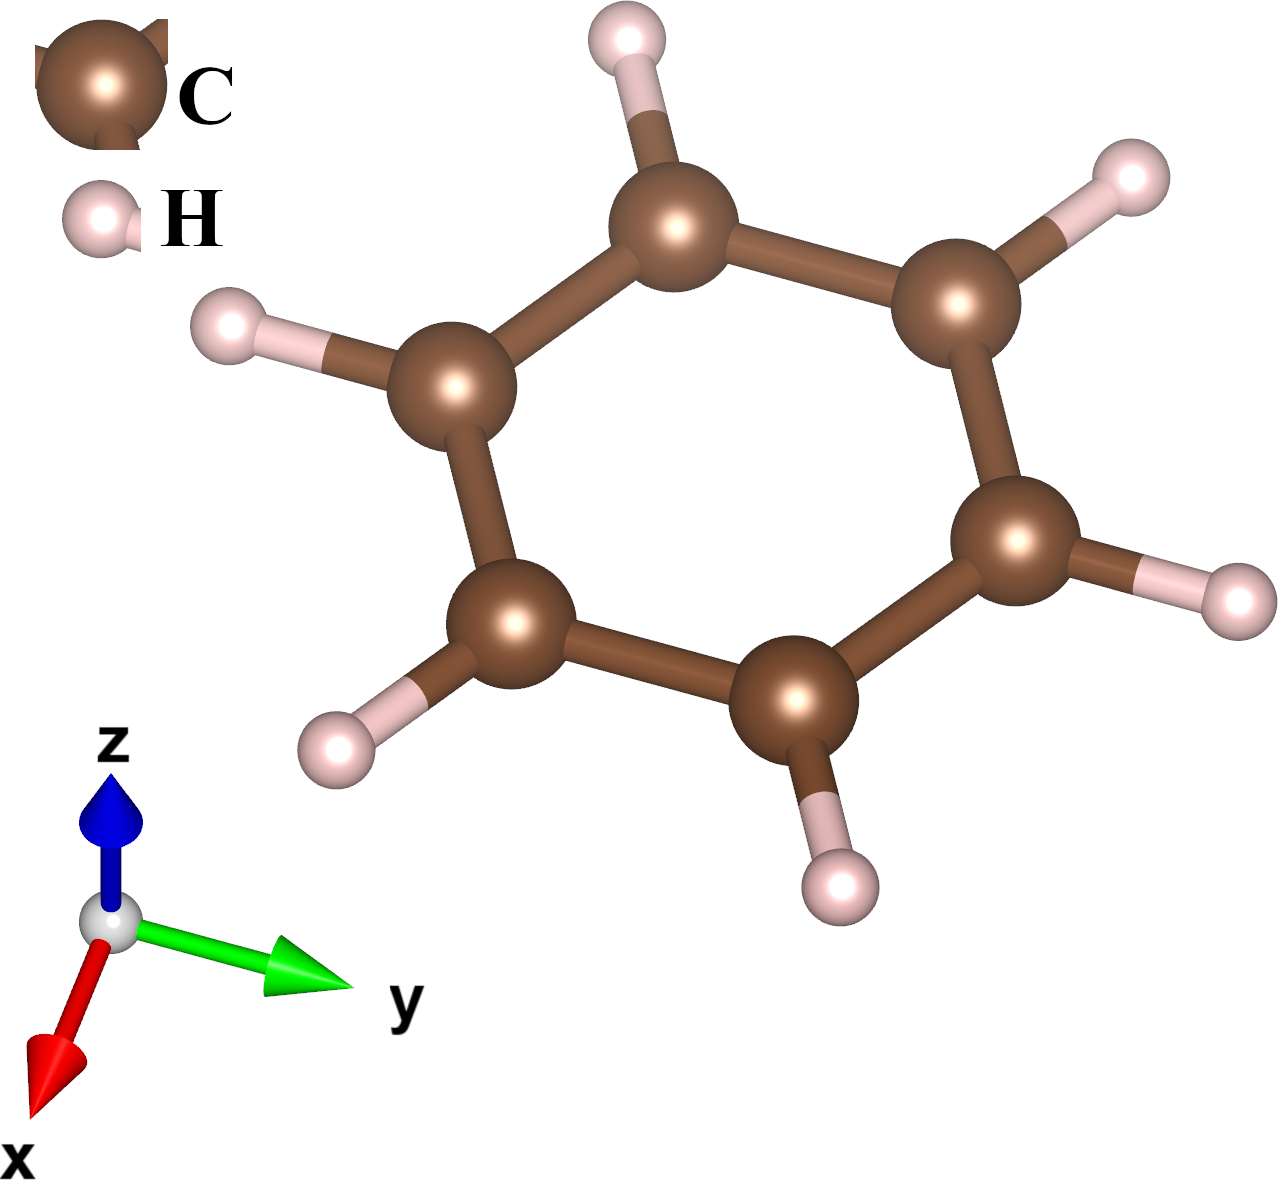
\includegraphics[width=5cm]{Benzene}
	%caption written between [ ] is shown in list of figure and caption
	%written between { } is shown just below the figure in the page
	\caption[C\tsb{6}H\tsb{6} structure]{Structure of Benzene (Created using
	VESTA \&\ edited with GIMP)}
	%add any unique variable between { } to use while refrencing
	\label{fig:benzene}
\end{figure}

This is an example of insterting multiple images in same line.

\begin{figure}[H]
	\centering
	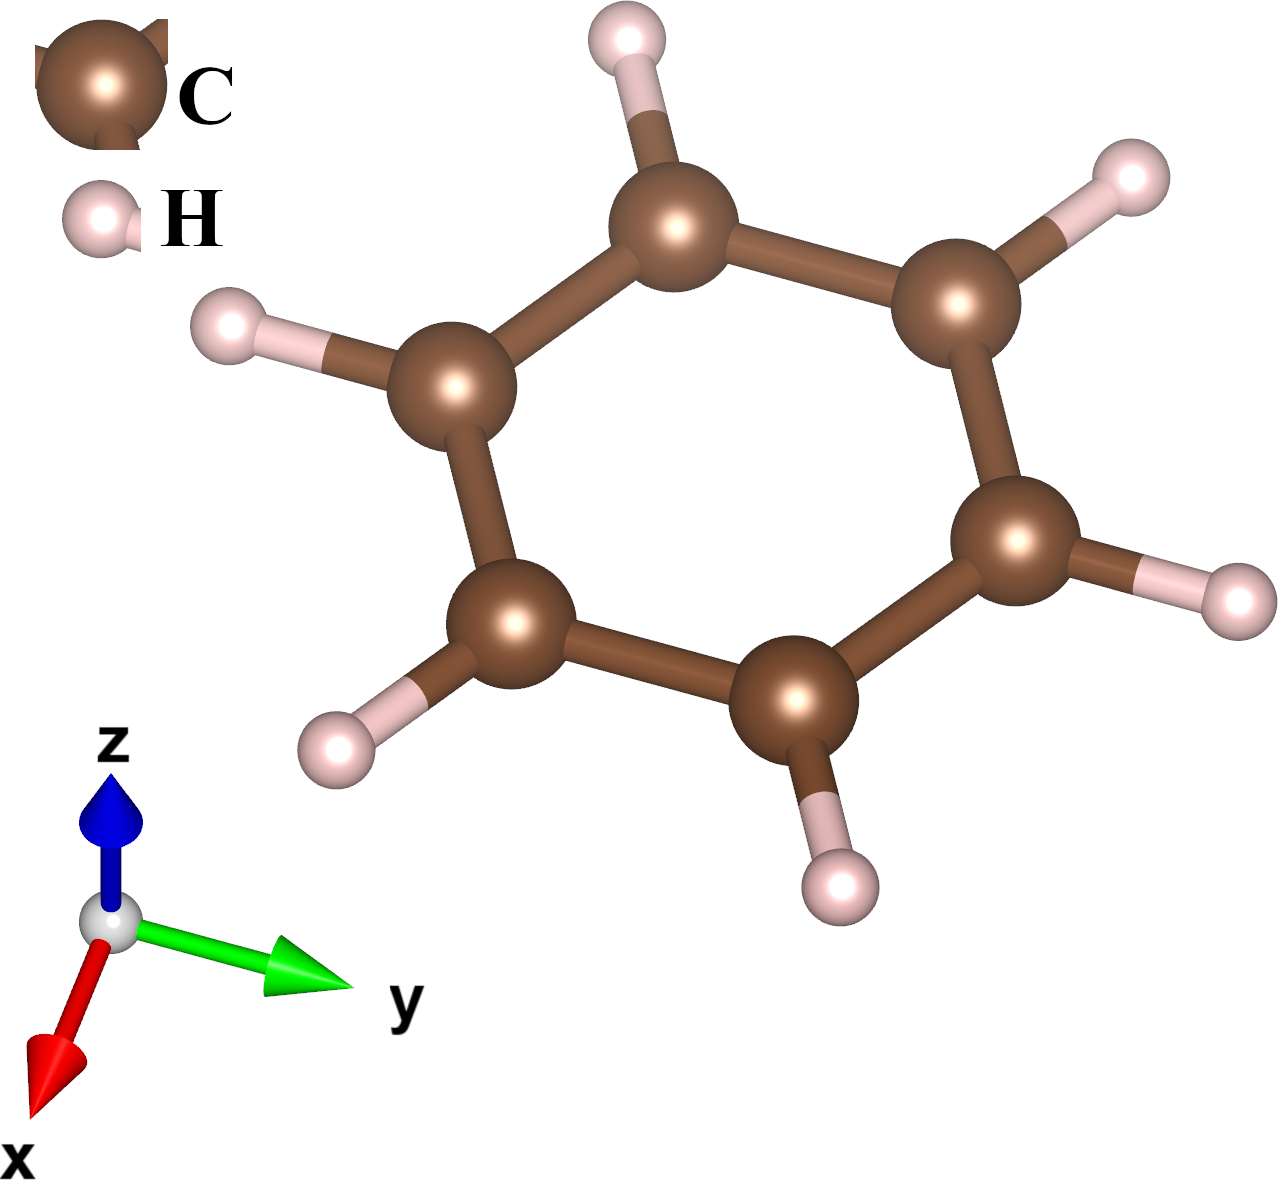
\includegraphics[width=5cm]{Benzene}
	\hspace{0.5cm}
	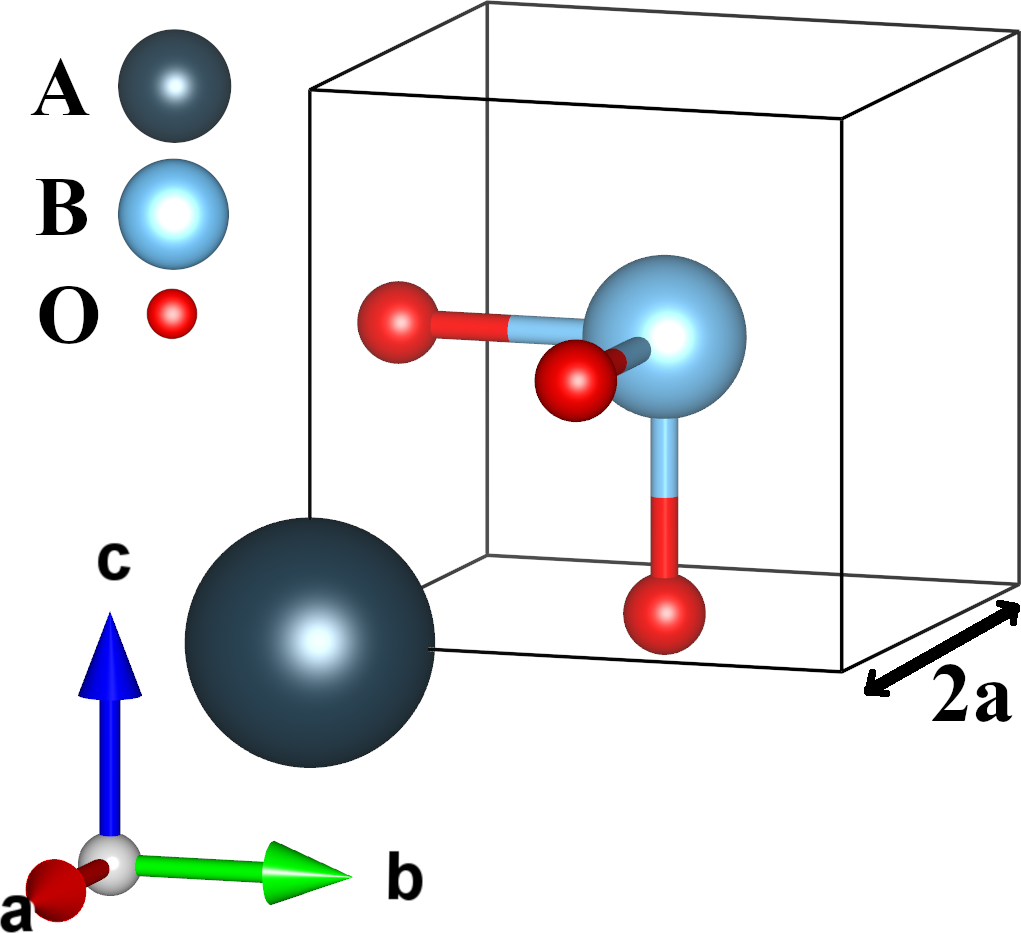
\includegraphics[width=5cm]{perovskite_unitcell}
	\caption[C\tsb{6}H\tsb{6} \&\ ABO\tsb{3} structure]{Structure of Benzene
	and Unit cell of perovskite (Created using VESTA \&\ edited with GIMP)}
\end{figure}

\section{Inserting Tables}

This is an example of insterting table.

\begin{table}[H] %[H] prints the table right at this position
	\centering
% | wtill vetical line separeting columns
% c means the component of the cell is centered 
\begin{tabular}{|c|c|c|c|}
	\hline %creates horizontal bar
	% & seperates the each componets of the cell
	Atoms & x & y & z\\ % \\ ends the row and start new row
	\hline
	A & 0.25 & 0.25 & 0.25\\
	% here we havent written hline so horizontal line wont show in table 
	B & 0.25 & 0.00 & 0.00\\
	C & 0.00 & 0.00 & 0.00\\
	D & 0.50 & 0.00 & 0.00\\
	\hline
\end{tabular}
	\caption[Atomic coordinates 1]{Atomic coordinates 1}
	\label{tab:atom}
\end{table}

This is an example of combining multiple column or multiple row in a table.

\begin{table}[H]
	\centering
\begin{tabular}{|c|c|c|c|}
	\hline
	% {2} represents merging ot 2 column in that row, {c|} mean center align
	Atoms & x & \multicolumn{2}{c|}{y \&\ z}\\
	\hline
	A  & 0.25 & 0.25 & 0.25\\
	\cline{2-4} % creates horizontal line from column 2 to 4
	{} & 0.25 & 0.00 & 0.00\\ % {} at the begining represents cell in empty
	\hline
	C  & 0.00 & 0.00 & 0.00\\
	\hline
	D  & 0.50 & 0.00 & 0.00\\
	\hline
\end{tabular}
	\caption[Atomic coordinates 2]{Atomic coordinates 2}
\end{table}

\section{Writing Equations}

This is an example for lengthy equation which doesn't fit in one line.
Use multline environment for this.

%add \\ where you want to break the equation and start from second line
\begin{multline}
	e^x = 1+x+\frac{x^2}{2!}+\frac{x^3}{3!}+\frac{x^4}{4!}+\frac{x^5}{5!}
	+\frac{x^6}{6!}+\frac{x^7}{7!}\\+\frac{x^8}{8!}+\frac{x^9}{9!}
	+\frac{x^{10}}{10!}+\frac{x^{11}}{11!}+\frac{x^{12}}{12!}
	+\frac{x^{13}}{13!}+\frac{x^{14}}{14!}+\cdots
	\label{eq:expansion}
\end{multline}

This is an example for writing multiple equations at a time.
Use align environment for this.

\begin{align}
	2x+6y&=64\\
	x+3y&=32
	\label{eq:xy}
\end{align}

\section{Referencing}

You can the bibtex citation key to put in reference.bib file in the site
Google Scholar.\\

Cite website and application like this: \hspace{1cm}
%put the variable from rerefence.bib file inbetween the { }
\cite{williams_gnuplot_nodate}

Cite articles and books like this: \hspace{1cm}
\cite{hohenberg1964inhomogeneous}

You can also put it inside square brackets like this: \hspace{1cm}
[\cite{hohenberg1964inhomogeneous}]   \\

You also can reference tables like this: \hspace{1cm} 
%put the variable you used in label inbetween \ref{ }
\textbf{Table \ref{tab:atom}}


You also can reference figure like this: \hspace{1cm} 
%put the variable you used in label inbetween \ref{ }
\textbf{Figure \ref{fig:benzene}}


You also can reference equations like this: \hspace{1cm} 
%put the variable you used in label inbetween \ref{ }
\textbf{Equation \ref{eq:expansion}} \\

\section{Using Acronymns/Symbols}

You can write acronyms/symbols as follow: \\

in short form like this \hspace{1cm}
%put the variable you used to denote the acronyms/symbols inbetween \acs{ }
\acs{t2g}

in long form like this \hspace{1cm}
%put the variable you used to denote the acronyms/symbols inbetween \acl{ }
\acl{lapw}

















%above file named example is just for example purpose, comment the above line

\chapter*{{\fontb CHAPTER 1\\} \fontc{1. INTRODUCTION}}

\pagenumbering{arabic} %using arabic style for page numbering

\pagenumbering{arabic} %using arabic style for page numbering

\chapter{INTRODUCTION}

\section{Heading}

\subsection{Sub-heading-1}

\subsection{Sub-heading-2}
	
\section{Rationale}

\section{Objective}

\subsection{General Objectives}

\subsection{Specific Objectives}





















\chapter*{{\fontb CHAPTER 2\\} \fontc{2. LITERATURE REVIEW}}

\toca{chapter}{\fonta{14}}{CHAPTER 2: LITERATURE REVIEW}

\tocb{section}{12}{2.1 Heading-1}


\tocb{section}{12}{2.2 Heading-2}



















\chapter*{{\fontb CHAPTER 3\\} \fontc{3. MATERIALS AND METHODS}}

\toca{chapter}{\fonta{14}}{CHAPTER 3: MATERIALS AND METHODS}

\tocb{section}{12}{3.1 Materials}

	\hspace{0.5cm}
	\tocb{subsection}{12}{3.1.1 Sub-heading-1}


	\hspace{0.5cm}
	\tocb{subsection}{12}{3.1.2 Sub-heading-2}

\tocb{section}{12}{3.2 Methods}

	\hspace{0.5cm}
	\tocb{subsection}{12}{3.2.1 Sub-heading-1}
	
	\hspace{0.5cm}
	\tocb{subsection}{12}{3.2.3 Sub-heading-2}





















\chapter*{{\fontb CHAPTER 4\\} \fontc{4. RESULTS AND DISCUSSION}}

\toca{chapter}{\fonta{14}}{CHAPTER 4: RESULTS AND DISCUSSION}

\tocb{section}{12}{4.1 Heading-1}

\tocb{section}{12}{4.2 Heading-2}




















\chapter*{{\fontb CHAPTER 5\\} \fontc{5. CONCLUSION AND RECOMMENDATION}}

\toca{chapter}{\fonta{14}}{CHAPTER 5: CONCLUSION AND RECOMMENDATION}

\tocb{section}{12}{5.1 Conclusions}


\tocb{section}{12}{5.2 Novelty and National Prosperity aspect of Project work}


\tocb{section}{12}{5.3 Limitaions of the work}


\tocb{section}{12}{5.4 Recomendations for the further work}

 



















\clearpage
\renewcommand{\bibname}{\fontb REFERENCE}% making title name REFERENCE
\toca{chapter}{\fonta{14}}{REFERENCE}% puting reference in TOC

\bibliographystyle{apalike}% using APA style for citation
\bibliography{reference}
\clearpage

\chapter*{\fontb APPENDIX\\}

\toca{chapter}{\fonta{14}}{APPENDIX}
















%%uncomment bottom 2 files if necessary only
%\newpage
\thispagestyle{empty} %makes it not show page number

\begin{center}

	\bfseries{
		\underline{\dn a\7{n}\8{s}cF{\rs -\re} 3 {\rs (\re}k{\rs )\re} }\\
		\vspace{10pt}
		\clz\\
		\depart\\
		\iost, \tu\\
		\vspace{0.3cm}
		\underline{Project Work Evaluation Form}
	}

\end{center}

\textbf{Name of Student:} \myname\\
\textbf{Title of Project work:} \title

\vspace{0.2cm}

Course Code: PRO-460 \hspace{1.5cm} Symbol No:\, \sym \hspace{1.5cm}
Date: . . . . . ./. . . . ./. . .

\vspace{0.2cm}

\textbf{Evaluation Scheme}

\vspace{5pt}

\begin{tabular}{|b{1cm}|b{3cm}|b{1cm}|b{3cm}|b{1cm}|b{3cm}|}
	\hline
	10 & Extraordinary & 9 & Excellent & 8 & Very Good \\ \hline
	7 & Good & 6 & Average & 5 & Poor\\ \hline
\end{tabular}

\vspace{5pt}
%\renewcommand{\arraystretch}{1.7}
\begin{tabular}{|l|b{0.4cm}|b{0.4cm}|b{0.4cm}|b{0.4cm}|b{0.4cm}|b{0.4cm}|l|}
	\hline
	\textbf{Evaluation Criteria} & \multicolumn{6}{|c|}
	{\textbf{{Evaluation (Circle One)}}} & \textbf{\parbox
	{3cm}{\fontsize{12pt}{10pt}\selectfont  \ \\Total Evaluated Number\\}}\\
	\hline
	Novelty & 10 & 9 & 8 & 7 & 6 & 5 & \multirow{10}{*}{}\\ \cline{1-7}
	Problem of Identification & 10 & 9 & 8 & 7 & 6 & 5 & \multirow{10}{*}{}\\
	\cline{1-7}
	Project Design & 10 & 9 & 8 & 7 & 6 & 5 & \multirow{10}{*}{}\\ \cline{1-7}
	Procedure, Data collection and analysis & 10 & 9 & 8 & 7 & 6 & 5 &
	\multirow{10}{*}{}\\ \cline{1-7}
	Conclusion and Future works & 10 & 9 & 8 & 7 & 6 & 5 & \multirow{10}{*}{}\\
	\cline{1-7}
	Literature review & 10 & 9 & 8 & 7 & 6 & 5 & \multirow{10}{*}{}\\
	\cline{1-7}
	Writing format & 10 & 9 & 8 & 7 & 6 & 5 & \multirow{10}{*}{}\\ \cline{1-7}
	Presentaion & 10 & 9 & 8 & 7 & 6 & 5 & \multirow{10}{*}{}\\ \cline{1-7}
	Viva-voce Performance & 10 & 9 & 8 & 7 & 6 & 5 & \multirow{10}{*}{}\\
	\cline{1-7}
	Social Impact & 10 & 9 & 8 & 7 & 6 & 5 & \multirow{10}{*}{}\\ \hline
\end{tabular}\\

Additional Comments (If any):

$$Marks\; obtained = {\frac{Total\; Evaluated\; Number}{100}}
\times {Full\; Marks\; of\; the\; Examiner}=$$

{\fontsize{9pt}{10pt}\selectfont
[F.M. for out of 100: Supervisor (40)/ External Examiner (25)/ Internal
Examiner(20)/ Head of the Department (15)]}

\vspace{5pt}

\textbf{Name:}\\
\textbf{Signature:}\\
\textbf{Date:}\\

\hrule

\vspace{5pt}

{\centering\textbf{Supervisor/External Examiner/Internal Examiner
/Head of the Department}\\}
























%\newpage
\thispagestyle{empty} %makes it not show page number

\begin{center}
	\bfseries{
	\underline{\fonts{16}{24}\preetiboldfont cg';"rL— \# -v\_}\\
	\vspace{10pt}
	Mark ledger of the Project work student
	}
\end{center}

\vspace{-1cm}

{\flushright{Date: . . . . . ./ . . ./ . . .}\\}

To,\\
The Office of the Controller of Examination,\\
B.Sc. Exam Section,\\
Tribhuvan University,\\
Balkhu, Kathmandu, Nepal.

\vspace{0.3cm}

{\centering\textbf{\underline{Subject: Marks of B.Sc. Project work (PRO 406)}}
\\}

Sir,

\hspace{1cm}Marks obtained by Mr.\;\myname\ (Batch 2075) for the
evaluation of Project
work conducted at the \depart, \clz for the partial fulfilment of B.Sc. in
\sub has been forwarded. The details are as follows:

\textbf{Year:}\ Fourth
\hspace{9cm}\textbf{Course Code:}\ PRO 406\\
\textbf{Full Marks: 100}
\hspace{9.5cm}\textbf{Pass Marks: 50}

\vspace{0.3cm}

\textbf{Title of Project work:} \title

\vspace{0.3cm}

Date of Submission : . . . . . . . . . . . . . . . . . . . . (BS)/
 . . . . . . . . . . . . . . . . . . . . (AD)\\
 Date of Viva-voce : . . . . . . . . . . . . . . . . . . . . (BS)/
 . . . . . . . . . . . . . . . . . . . . (AD)\\

\begin{tabular}{|l|l|l|l|l|b{4.5cm}|}
	\hline
	S.N. & Symbol No. & Registration No. & Name of Student & \parbox{4.5cm}
	{\fontsize{12pt}{10pt}\selectfont\ \\Marks obtained (In figure\\and words)}
	\\ \hline
	1. & \sym & \reg & \myname & \parbox{4.5cm}{\vspace{1cm}}
	\\ \hline
\end{tabular}\\

\vspace{0.3cm}

Name and Signature of the members of Projects work Evaluation committee/Board:

\begin{tabular}{|l|m{5.5cm}|m{4cm}|}
	\hline
	& Name & Signature \\ \hline
	Supervisor: & \sup & \\ \hline
	Co-supervisor: & \cosup & \\ \hline
	External Examiner: & & \\ \hline
	Internal Examiner: & & \\ \hline
	Head of the Department: & \hod & \\ \hline
\end{tabular}

{\flushright{
	\hod\\
	Head of the Department\\
	\clz
}\\
}
















%%uncomment above 2 files if necessary only

}

\end{document}



















